% Simplified User Flow Diagram (Alternative Version)
% Requires: \usepackage{tikz}
% Simpler, more linear flow

\begin{figure}[h]
\centering
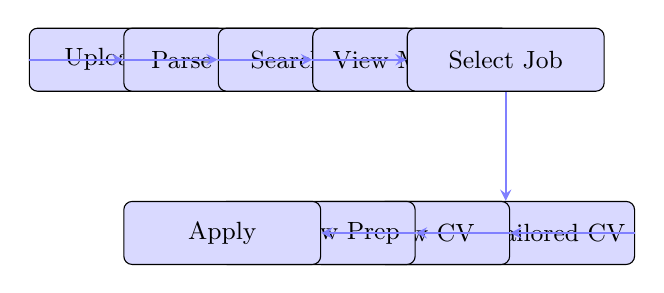
\begin{tikzpicture}[
    node distance = 1.2cm,
    auto,
    block/.style = {
        rectangle,
        rounded corners = 3pt,
        minimum width = 2.5cm,
        minimum height = 0.8cm,
        text centered,
        draw = black,
        fill = blue!15,
        font = \small
    },
    arrow/.style = {
        ->,
        >=stealth,
        thick,
        blue!50
    }
]

    % Nodes
    \node [block] (1) {Upload CV};
    \node [block, right of = 1] (2) {Parse Profile};
    \node [block, right of = 2] (3) {Search Jobs};
    \node [block, right of = 3] (4) {View Matches};
    \node [block, right of = 4] (5) {Select Job};
    \node [block, below of = 5, yshift = -1cm] (6) {Generate\\Tailored CV};
    \node [block, left of = 6] (7) {Review CV};
    \node [block, left of = 7] (8) {Interview Prep};
    \node [block, left of = 8] (9) {Apply};
    
    % Arrows
    \draw [arrow] (1) -- (2);
    \draw [arrow] (2) -- (3);
    \draw [arrow] (3) -- (4);
    \draw [arrow] (4) -- (5);
    \draw [arrow] (5) -- (6);
    \draw [arrow] (6) -- (7);
    \draw [arrow] (7) -- (8);
    \draw [arrow] (8) -- (9);
    
\end{tikzpicture}
\caption{Simplified User Flow: Job Application Process}
\label{fig:user_flow_simple}
\end{figure}

